\subsection{Redesigning the Database Model}\label{databaseModelRedesignNF}
We will now create relations describing the new models for the database.
Other groups of the \knox{} pipeline have requested that entities representing articles have a unique Id field, regardless of what is considered good database design.
Similarly, they want a field denoting the total words appearing in the article.

We will start by creating an ER-model of the domain, and then describe the entity and relationship sets using the relational model, using the method described in section \ref{relational_databases}.

\begin{figure}[H]
    \centering
    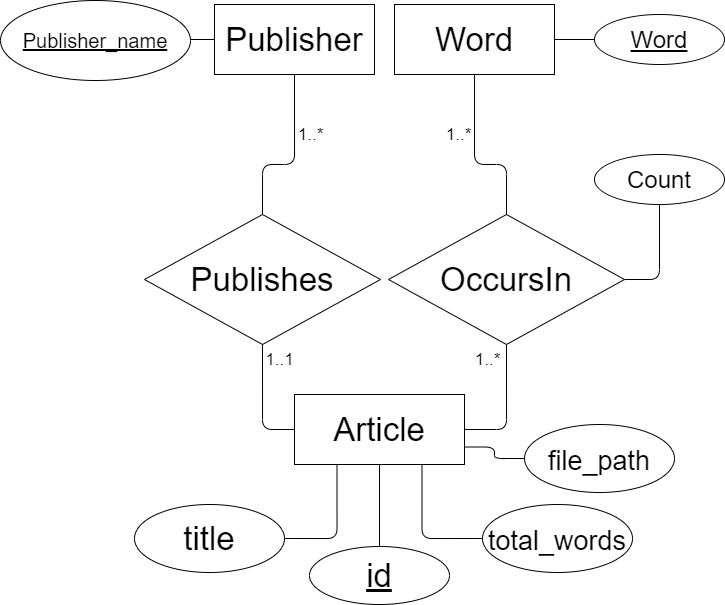
\includegraphics[scale=0.35]{Images/new ER.drawio.png}
    \caption{ER diagram depicting the new model of the database. Notice that the relationship set \textit{Publishes} and entity set \textit{publisher} has not changed.}
    \label{fig:newdatabaseRedesignER}
\end{figure}

Equation \ref{eq:newDatabaseRelationalModel} shows relations representing the new database structures from figure \ref{fig:newdatabaseRedesignER}.
Notice that the existing $publisher$ relation in the database have exactly the same attributes as the new one. 

\begin{equation}\label{eq:newDatabaseRelationalModel}
    \begin{split}
        article(\underline{article\_id: \mathbb{Z^+}}, title:text,\\ total\_words:\mathbb{Z^+}, publisher\_name \rightarrow publisher, file\_path:text), \\
        word(\underline{text:text}),\\
        publisher(\underline{publisher\_name:text}),\\
        occursIn(\underline{text \rightarrow word}, \underline{article\_id \rightarrow article}, count:\mathbb{Z^+})\\
    \end{split}
\end{equation}


We have to ensure that the WordRatio view, described in section \ref{WordRatioCrud} and appendix \ref{Appendix_WordRatioOld}, still contains the same information as before.
Since the view is an abstraction over a \texttt{SELECT} query, we will describe it using relational algebra.
The query of the view can be seen in equation \ref{create_new_view_rel_alg}.
The resulting relation structure is seen in equation \ref{create_new_view_rel_alg_structure}.


\begin{equation}\label{create_new_view_rel_alg}
    \begin{split}
        \sigma_{article\_id, text, count,title, file\_path, total\_words, publisher\_name, percent} \\
        ((article \Join_{article.article\_id = occursIn.article\_id} occursIn) \\
        \Join_{article.publisher\_name = publisher.publisher\_name} publisher\\
        \Join \gamma_{article, occursIn;percent(count, total\_words)})
    \end{split}
\end{equation}

\begin{equation}\label{create_new_view_rel_alg_structure}
    \begin{split}
        wordRatio(article\_id:\mathbb{Z^+}, text:text, count:\mathbb{Z^+},title:text, file\_path:text,\\ total\_words:\mathbb{Z^+}, publisher\_name:text, percent:\mathbb{R^+})
    \end{split}
\end{equation}


